\documentclass[aspectratio=169,xcolor=dvipsnames]{beamer}
\usepackage{ods}

\title{Interfaces/Abstract Data Types}
\author{Open Data Structures}
\titlegraphic{}
\titlegraphic{
\includegraphics[height=1em]{by}}

\begin{document}

\begin{frame}
  \titlepage
\end{frame}

\begin{frame}
  \frametitle{Interfaces/Abstract Data Types}
 
  \begin{itemize}
   \item<+->Describes what a data structure \emph{does}:
     \begin{itemize}
        \item<+->supported operations (the \emph{interface})
        \item<+->meaning of operations (the \emph{semantics})
     \end{itemize}
   \item<+-> \sout{Representation and implementation}
        \end{itemize}
\end{frame}

\begin{frame}
  \frametitle{Abstract Data Types/Interfaces}

  \begin{tabular}{p{.3\textwidth}p{.6\textwidth}}
  \raisebox{-.5\height}{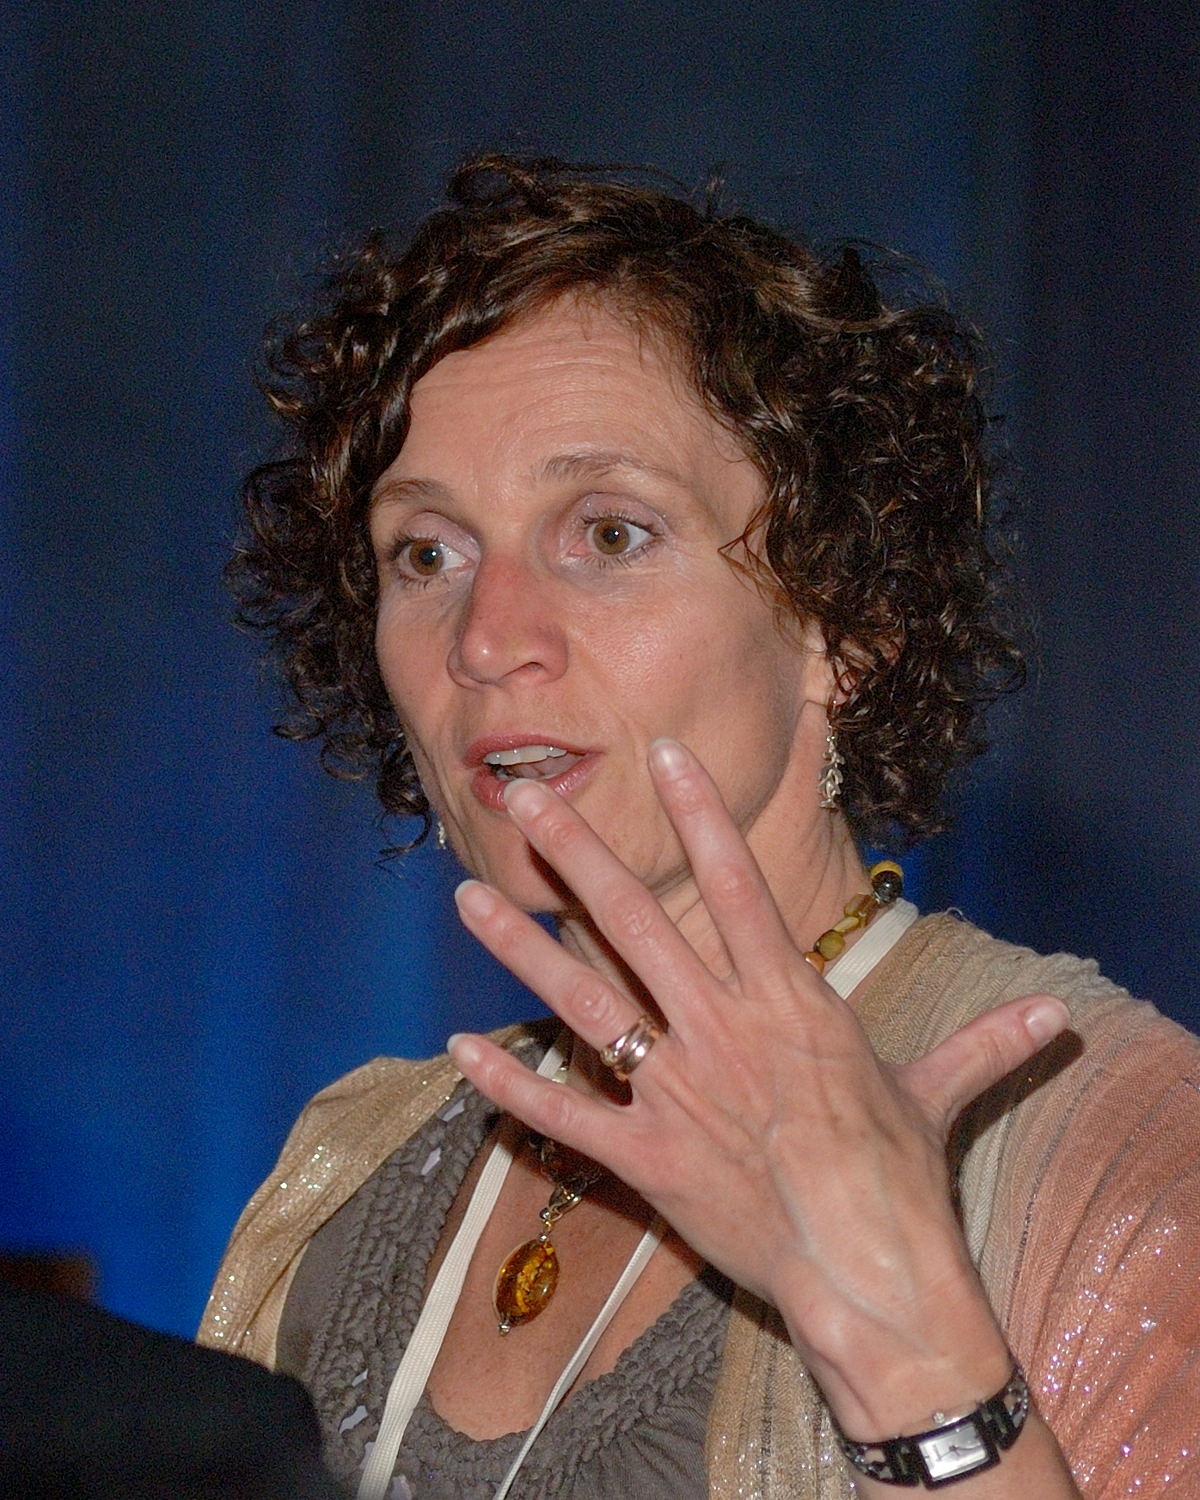
\includegraphics[width=.28\textwidth]{images/liskov}} \newline\newline
  \raggedright   Barbara Liskov at the ACM Turing Centenary Celebration
  \mbox{(\copyright~2012~Dennis~Hamilton)}
 &

   \raggedright 
   \only<+->{B. Liskov and S. N. Zilles, Programming with Abstract Data Types, \emphen{SIGPlan Notices}, 9(4), pp. 50-59, 1974.\\}
   \only<+->{abstract data type $=$ interface}
  \end{tabular}
\end{frame}

\closing

\end{document}

